% !TEX program = xelatex
\documentclass[aspectratio=169]{beamer}
\makeatletter
\def\@makefnmark{}
\makeatletter
\usepackage{amsthm,amsmath,amssymb,braket,fontspec,unicode-math}
\usepackage[absolute,overlay]{textpos}
\usetheme[numbering=none]{focus}
\setbeamercolor{footnote}{fg=azure}
\setbeamerfont{footnote}{size=\tiny,series=\bfseries}
\setbeamerfont{alerted text}{series=\bfseries}

\setmathfont{Latin Modern Math}[range={frak,\bigcap,\bigcup}]

\setmathfont{Latin Modern Math}[range=\checkmark]

\usepackage[backend=bibtex,url=false,doi=false,maxcitenames=1, style=authoryear]{biblatex}
\bibliography{bib}
\AtBeginBibliography{\scriptsize}

\newcommand{\focus}[1]{\textcolor{red}{\bf{#1}}}
\AtBeginSection[]{}
\definecolor{red}{HTML}{CC0000}
\definecolor{lred}{HTML}{e24a33}
\definecolor{bgreen}{HTML}{006A4E}
\definecolor{azure}{HTML}{007fff}
\newcommand{\alertb}[1]{\color{azure}\alert{#1}}
\setbeamertemplate{bibliography item}[triangle]

\graphicspath{{./figures/}}

%\AtBeginSection[]{
%  \vfill
%  \centering
%  \begin{beamercolorbox}[sep=20pt,rounded=true,center]{frametitle}
%    \usebeamerfont{title}\insertsectionhead\par%
%  \end{beamercolorbox}
%  \vfill
%}
\title{\LARGE Emergence in correlated fermions: From impurity models to the bulk}

\author{\textbf{Abhirup Mukherjee}\\\alert{RPC Presentation 2022-2023}}
\institute{\textbf{Emergent Phenomena in Quantum Matter} Group\\
Department of Physical Sciences, IISER Kolkata}

\date{July 11, 2023}
\begin{document}

\centering

\begin{frame}
\maketitle
\begin{textblock*}{0.13\textwidth}(13.5cm, 4.3cm)
	\centering

	\includegraphics[width=\textwidth]{epqm_logo_mod.jpeg}\\
	\vspace*{\fill}
	\includegraphics[width=\textwidth]{dps_logo.jpeg}
\end{textblock*}
\end{frame}

\begin{frame}{}
\hspace*{\fill}
\begin{minipage}{0.1\textwidth}
	\includegraphics[width=\textwidth]{epqm_logo_mod.jpeg}
\end{minipage}
\begin{minipage}{0.22\textwidth}
	\centering
	\includegraphics[width=0.6\textwidth]{slal.jpg}\\
	\footnotesize{{\bf Siddhartha Lal}\\
	}
\end{minipage}
\begin{minipage}{0.22\textwidth}
	\centering
	\includegraphics[width=0.6\textwidth]{amukherjee.jpg}\\
	\footnotesize{{\bf Anirban Mukherjee}\\
	}
\end{minipage}
\begin{minipage}{0.22\textwidth}
	\centering
	\includegraphics[width=0.6\textwidth]{spatra.jpeg}\\
	\footnotesize{{\bf Siddhartha Patra}\\
	}
\end{minipage}
\begin{minipage}{0.1\textwidth}
	\includegraphics[width=\textwidth]{dps_logo.jpeg}
\end{minipage}
\hspace*{\fill}
\\
\vspace*{\fill}
\begin{minipage}{0.1\textwidth}
\includegraphics[width=\textwidth]{IISER-K.png}
\end{minipage}
\hspace*{\fill}
\begin{minipage}{0.6\textwidth}
\centering
\alert{$\sim\sim\sim\sim\sim\sim\sim\sim\sim\sim\sim\sim\sim\sim\sim$ }\\
\alert{A huge thanks to all my collaborators! }\\
\alert{Thanks to IISER K and SERB for financial support.}\\
\alert{$\sim\sim\sim\sim\sim\sim\sim\sim\sim\sim\sim\sim\sim\sim\sim$ }\\
\end{minipage}
\hspace*{\fill}
\begin{minipage}{0.15\textwidth}
\includegraphics[width=\textwidth]{SERB.png}
\end{minipage}
\vspace*{\fill}

\hspace*{\fill}
\begin{minipage}{0.1\textwidth}
	\includegraphics[width=\textwidth]{IITKGP.png}\\
\end{minipage}
\hspace*{\fill}
\begin{minipage}{0.3\textwidth}
	\centering
	\includegraphics[width=0.4\textwidth]{arghya.jpg}\\
	\footnotesize{{\bf Arghya Taraphder}\\
	IIT Kharagpur}
\end{minipage}
\hspace*{\fill}
\begin{minipage}{0.3\textwidth}
	\centering
	\includegraphics[width=0.4\textwidth]{nsv.jpeg}\\
	\footnotesize{{\bf N. S. Vidhyadhiraja}\\
	JNCASR Bangalore}
\end{minipage}
\hspace*{\fill}
\begin{minipage}{0.1\textwidth}
	\includegraphics[width=\textwidth]{JNCASR.png}\\
\end{minipage}
\hspace*{\fill}

\end{frame}

\section{List of completed and ongoing projects}
\subsection{~}

\begin{frame}{List of publications, preprints and ongoing projects}
\only<1-2>{
\begin{itemize}
	\item[$\checkmark$] \onslide<1->{Unveiling the Kondo cloud: Unitary RG study of the Kondo model.\\  2022 \alert{Phys. Rev. B} 105, 085119.\\ A Mukherjee, \alert{Abhirup Mukherjee}, N. S. Vidhyadhiraja, A. Taraphder, S Lal\\[10pt]}
	\item[$\checkmark$] \onslide<1->{Frustration shapes multi-channel Kondo physics: a star graph perspective.\\  2023 \alert{J. Phys.: Condens. Matter} 35 315601. \\ S Patra, \alert{Abhirup Mukherjee}, A Mukherjee, N. S. Vidhyadhiraja, A Taraphder, S Lal\\[10pt]
	}
\item \onslide<2->{Kondo frustration via charge fluctuations: a route to Mott localisation.\\  2023 arXiv:2302.02328. \alert{under review} at New Journal of Physics.\\ \alert{Abhirup Mukherjee}, N. S. Vidhyadhiraja, A. Taraphder, S Lal\\[10pt]}
\item \onslide<2->{Holographic entanglement renormalisation for fermionic quantum matter.\\ 2023 arXiv:2302.10590. \alert{under review} at Journal of HEP.\\ \alert{Abhirup Mukherjee}, S Patra, S Lal
	}
\end{itemize}
}
\only<3>{
\vspace*{-30pt}
\flushleft
\alert{Currently in progress}\\
\begin{itemize}
	\item Development of auxiliary model-based method for studying bulk correlated systems.\\[10pt]
	\item Studies of the plateau-to-plateau transition in integer quantum hall systems.
\end{itemize}

\vspace*{20pt}
\hrule

\vspace*{\fill}
\begin{minipage}{0.55\textwidth}
\begin{itemize}
	\item[$\checkmark$] 2022 \alert{Phys. Rev. B} 105, 085119.\\ A Mukherjee, \alert{Abhirup Mukherjee}, \ldots, S. Lal\\[10pt]
	\item[$\checkmark$] 2023 \alert{J. Phys.: Condens. Matter} 35 315601.\\ S Patra, \alert{Abhirup Mukherjee}, \ldots, S. Lal
\end{itemize}
\end{minipage}
\begin{minipage}{0.44\textwidth}
\begin{itemize}
	\item 2023 \alert{arXiv:2302.02328}.\\ \alert{Abhirup Mukherjee}, \ldots, S. Lal\\[10pt]
	\item 2023 \alert{arXiv:2302.10590}.\\ \alert{Abhirup Mukherjee}, \ldots, S. Lal
\end{itemize}
\end{minipage}
}

\end{frame}

\section{Quantum phase transition in an extended-SIAM}
\subsection{Abhirup Mukherjee, N. S. Vidhyadhiraja, A. Taraphder, Siddhartha Lal\\ arXiv:2302.02328. (2023)}

\begin{frame}{Some broad questions}
\only<1>{
\begin{minipage}{0.44\textwidth}
Dynamical mean-field theory shows \alert{metal-insulator transition} for the Hubbard model in \(\infty\) dimensions.
\end{minipage}
\hspace*{\fill}
\begin{minipage}{0.48\textwidth}
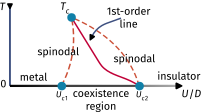
\includegraphics[width=0.9\textwidth]{coexistence-dmft.pdf}
\end{minipage}

\vspace*{\fill}
\flushleft
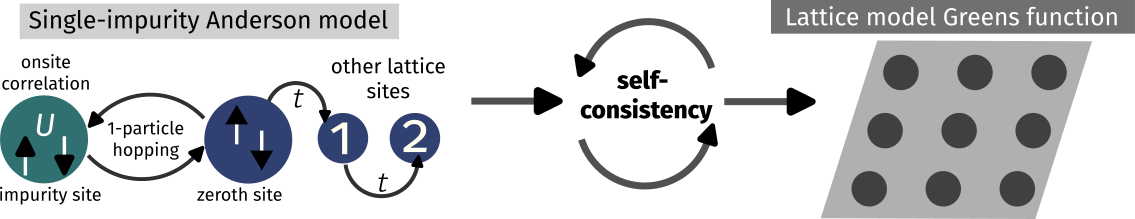
\includegraphics[width=\textwidth]{selfconsistency.pdf}
}

\only<2>{
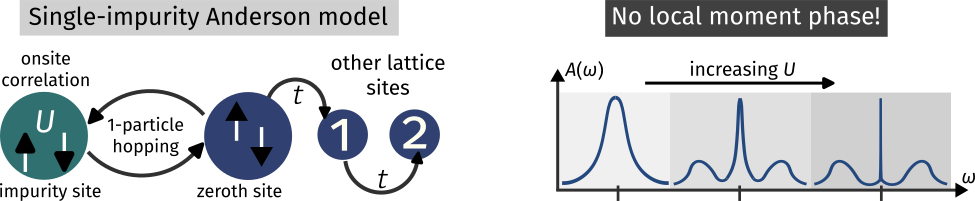
\includegraphics[width=\textwidth]{siam_schematic.pdf}

\vspace*{\fill}
Standard Anderson model shows \alert{no transition}, can't explain DMFT phase diagram.

\vspace*{\fill}
\begin{itemize}
	\item Which impurity model is realised through self-consistency?\\[10pt]
	\item What physics leads to \(U_{c1}\) and \(U_{c2}\)?\\[10pt]
	\item What is the state precisely at the \(T=0\) transition?
\end{itemize}
}

\end{frame}

\begin{frame}{Results}
	
\end{frame}

\section{Holography of entanglement in 2D free fermions}
\subsection{Abhirup Mukherjee, Siddhartha Patra, Siddhartha Lal\\ arXiv:2302.10590. (2023)}

\section{Tiling the lattice with the extended SIAM}
\subsection{Ongoing project}

\section{Search for punctured-Chern topology at IQHE transitions}
\subsection{Ongoing project}

\section{The extended-SIAM project}
\subsection{Abhirup Mukherjee, N. S. Vidhyadhiraja, A. Taraphder, S. Lal\\ arXiv:2302.02328. (2023)}

\begin{frame}{What is the new physics ingredient?}
\footcite{kotliar1992}
\begin{minipage}{0.39\textwidth}
	Add \alert{local correlation} on bath (zeroth) site coupled to impurity
\[KE_\text{bath} + J \vec{S}_\text{imp}\cdot\vec{S}_\text{bath} - U_b\left( \vec{S}_\text{bath} \right)^2 \]
\end{minipage}
\hspace*{\fill}
\begin{minipage}{0.55\textwidth}

\includegraphics[width=\textwidth]{zeromode_bare.pdf}
\end{minipage}

\vspace*{\fill}
URG equations show that an \alert{attractive} \(U_b\) frustrates the zeroth site.
\[\Delta J \sim J^2 + 4U_b J \implies \text{\alert{phase transition} at }J = -4U_b\]

\vspace*{\fill}
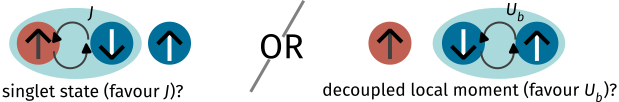
\includegraphics[width=0.9\textwidth]{frustration.pdf}\\

\vspace*{\fill}
Such a model sheds light on the Mott MIT in \(\infty-\)dimensions (as seen from DMFT).
\end{frame}

\begin{frame}{Nature of the transition}
\begin{minipage}{0.45\textwidth}
Across the transition,\\
\begin{itemize}
	\item impurity correlations vanish
	\item bath correlations become non-zero\\[10pt]
\end{itemize}

Shows that \alert{pairing correlations} in the bath are responsible for the transition.
\end{minipage}
\hspace*{\fill}
\begin{minipage}{0.5\textwidth}
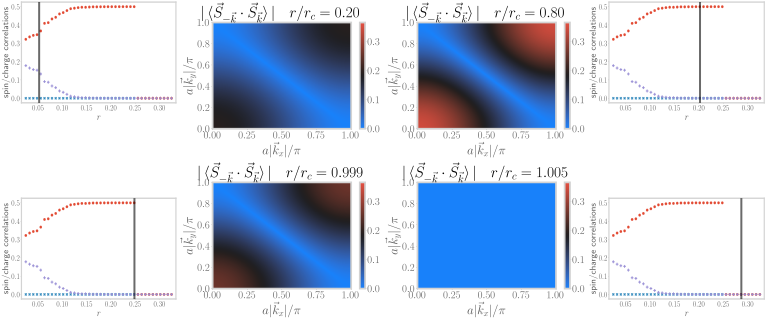
\includegraphics[width=\textwidth]{spin-charge-corr-full.pdf}
\end{minipage}

\vspace*{\fill}
The state \alert{precisely at the transition} is special:
\begin{itemize}
	\item non-Fermi liquid excitations
	\item \alert{fractional} impurity magnetisation and occupancy
\end{itemize}
\end{frame}

\section{Concluding remarks}
\subsection{~}

\begin{frame}{}
	\begin{itemize}
	\item Our analyses often link entanglement measures with correlations, providing bridges between the worlds of condensed matter and quantum information.\\[10pt]
	\item Models of Kondo breakdown can be used to study the effects of measurement on a system coupled to a bath.\\[10pt]
	\begin{center}
	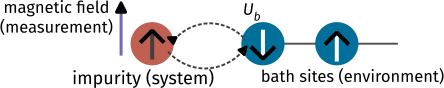
\includegraphics[width=0.5\textwidth]{measurement.pdf}
	\end{center}
	\item The Kondo model with attractive \(U_b\) term has applications in studying the physics of Mott transitions.
\end{itemize}
\end{frame}

\begin{frame}
	
\includegraphics[width=0.65\textwidth]{thanks.pdf}
\end{frame}

\begin{frame}{How to explain the resistance minimum \& eventual saturation?}
\footcite{kondo1964resistance}
\begin{minipage}{0.5\textwidth}
Second order perturbation theory in \(J\) gives:
\[\hspace*{-80pt}\rho \sim T^n - \ln T\]
Explains the \alert{non-monotonic}\\
behaviour!\\[20pt]
However, solution \alert{diverges} at \(T \to 0\)!
\end{minipage}
\begin{minipage}{0.4\textwidth}
	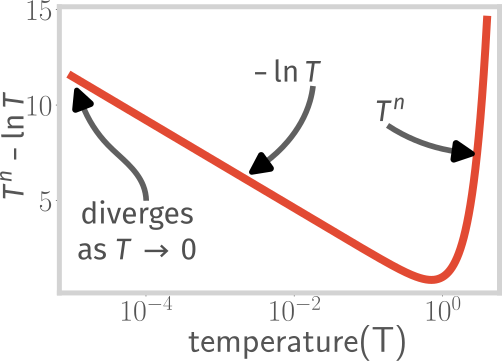
\includegraphics[width=\textwidth]{secondorder.pdf}
\end{minipage}
\begin{textblock*}{0.13\textwidth}(6.5cm, 3.8cm)
	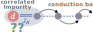
\includegraphics[width=\textwidth]{kondo.jpg}\\
	\footnotesize{(Jun Kondo)}
\end{textblock*}
\end{frame}


\begin{frame}{Unitary RG approach to impurity models}
\footcite{anirbanurg1,anirbanurg2}
\begin{minipage}{0.5\textwidth}
\begin{itemize}
	\item Integrate out \alert{high energy fluctuations} to reach strong-coupling low-energy theory\\[10pt]
	\item Leads to \alert{singlet ground state} and decoupled high-energy \(k-\)states\\[10pt]
	\item Decoupling is carried out through \alert{unitary transformations}
\end{itemize}

\end{minipage}
\hspace*{\fill}
\begin{minipage}{0.4\textwidth}
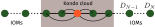
\includegraphics[width=\textwidth]{kondo_fp_1D.pdf}
\end{minipage}
	
\end{frame}

\begin{frame}
\begin{minipage}{0.8\textwidth}
\end{minipage}

\vspace*{\fill}
\begin{itemize}[<+->]
	\item Entanglement entropy \(S(A)\) \(\Longrightarrow\) quantifies how much \alert{information is gained} about the rest of the system by measuring \(A\)\\
	\vspace*{\fill}
	{\centering
	\only<1>{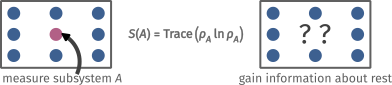
\includegraphics[width=0.85\textwidth]{entanglement.pdf}}}
\item Mutual information \(I_2(A:B)\)\(\Longrightarrow\) quantifies how much \alert{information about subsystem A} is gained by measuring \(B\)\\
	\vspace*{\fill}
	{\centering
	\only<2>{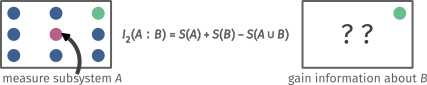
\includegraphics[width=0.85\textwidth]{mutinfo.pdf}}}
\end{itemize}
\end{frame}
\end{document}
